\section{Function Merging} \label{sec:fm}

In this section, we describe the proposed function-merging technique.
Contrary to the state-of-the-art, our technique is able to merge any two
functions.
If the two functions are equivalent, i.e., identical, then the two functions
can be completely merged into a single identical function.
However, if the two functions differ at any point, an extra parameter is
required, so that the caller is able to distinguish between the functions. 
The two functions can differ in any possible way, including their list of
parameters or return types.
If the lists of parameters are different, we can merge them so that we are able
to uniquely represent all parameters from both functions.
If the return types are different, we can use an aggregate type to return values
of both types or return just the non-void type if the other one is void.
%However, in our current implementation, the only restriction is that both
%functions must have equivalent return types or one of them must be \textit{void}.

\begin{figure}[h]
  \centering
  %\vspace{-1ex}
  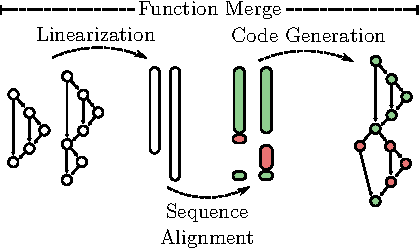
\includegraphics[width=0.85\linewidth]{figs/func-merge-overview.pdf}
  \caption{Overview of our function-merging technique.}
  \label{fig:func-merge-overview}
  %\vspace{-1ex}
\end{figure}

The proposed technique consists of three major steps, as depicted in
Figure~\ref{fig:func-merge-overview}.
First, we linearize each function, representing the CFG as a sequence of 
labels and instructions.
The second step consists in applying a sequence alignment algorithm, borrowed
from bioinformatics, which identifies regions of similarity between sequences.
The sequence alignment algorithm allows us to arrange two linearized functions
into segments that are equivalent between the two functions and segments where
they differ from one another.
The final step performs the code generation, actually merging the two functions
into a single function based on the aligned sequences.
Aligned segments with equivalent code are merged, avoiding redundancy, %redundant code,
and the remaining segments where the two functions differ have their code
guarded by a function identifier.
At this point, we also create a merged list of parameters where parameters of
the same type are shared between the functions, without necessarily keeping
their original order.
This new function can then be used to replace the original functions, as they
are semantically equivalent, given the appropriate function-identifier
parameter.

\subsection{Linearization}

The \textit{linearization}\footnote{Although linearization of CFGs
usually refers to a predicated representation, % resulting from an if-conversion,
in this paper, we refer to a simpler definition.}
of a function consits in specifying an ordering of the basic blocks based on a
traversal of the CFG and then producing a sequence of basic block labels and
instructions, similar to a textual representation of the function.
Although this operation is trivial, the specific ordering of the basic blocks
chosen can have an impact on the merging operation.

%For the linearization, we assume that every basic block has an entry label and
%a terminator instruction which refers explicitly to the successor basic blocks,
%if there are successors.
%This is true for most IRs, such as the LLVM IR, or can be easily adapted.

In our implementation, the linearization uses a reverse post-order~(RPO) of the
basic blocks, following a canonical ordering of the successors.
%, e.g., \textit{true} branches before \textit{false} ones.
%Figure~\ref{fig:branch-linearization} shows an example of the linearization 
%using the canonical RPO.
The RPO guarantees that the linearization starts with the entry basic block and
then proceeds favoring definitions before uses, except in the presence of loops.
Although the specifc ordering produced by the canonical linearization may not
be optimal, it is common practice for compilers to rely on prior
canonicalizations, e.g., 
canonical loops, canonical induction variables, canonical reassociation, etc.
For contrast, if, instead, we use an RPO linearization with a uniformly
randomized ordering of the successor basic blocks, the final code-size reduction
of the function-merging optimization can drop up to 10\% for individual
benchmarks.
Note that our decision for using the canonical RPO is purely pragmatic and
other orderings of the basic blocks could also be used, as long as it produces
a sequence of labels followed by instructions.

%\begin{figure}[h]
%  \centering
%  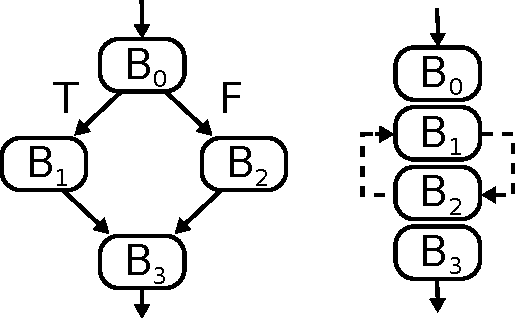
\includegraphics[width=0.6\linewidth]{figs/branch-linearization.pdf}
%  \caption{Linearization using a canonical reverse post-order.
%           The dashed arrows show where a randomized ordering could change the
%           linearization.}
%  \label{fig:branch-linearization}
%\end{figure}

\subsection{Sequence Alignment}

When merging two functions, the goal is to identify which pairs of instructions
and labels that can be merged and which ones need to be selected based on the
actual function being executed.
To avoid breaking the semantics of the original program, we also need to
maintain the same order of execution of the instructions for each one of
the functions.

To this end, after linearization, we reduce the problem of merging functions
to the problem of \textit{sequence alignment}. %~\cite{carrillo88,wang94}.
%After linearization, the problem of merging two functions can be reduced to the
%\textit{sequence alignment} problem~\cite{carrillo88,wang94}, which is itself
%closely related to finding the
%\textit{longest common subsequence}~\cite{hirschberg75,maier78}.
Sequence alignment is an important technique to many areas of science,
most notably in molecular biology~\cite{needleman70,smith81,carrillo88,wang94}
where, for example, it is used for identifying homologous subsequences of amino
acid in proteins.
Figure~\ref{fig:opcode-align} shows an example of the sequence alignment
between two linearized functions extracted from the \text{400.perlbench} benchmark
in SPEC CPU2006~\cite{spec}.

\begin{figure}[h]
  \centering
  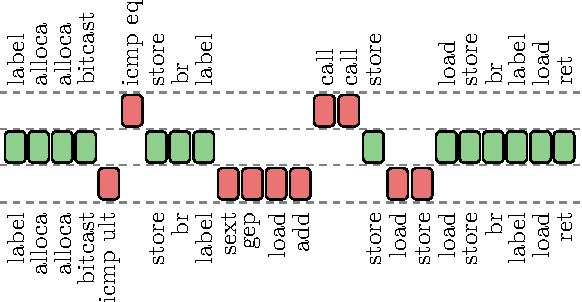
\includegraphics[width=0.85\linewidth]{figs/opcode-align.pdf}
  %\caption{An example of a sequence alignment between two real functions extracted from the \text{400.perlbench} benchmark.}
  \caption{The sequence alignment between two functions.}
  \label{fig:opcode-align}
\end{figure}

Formally, sequence alignment can be defined as follows:
For a given alphabet $\alpha$, a sequence $S$ of $k$ characters is a subset of
$\alpha^k$, i.e., $S = (a_1, \ldots a_k)$.
Let $S_1, \ldots, S_m$ be a set of sequences, possibly of different lengths but
all derived from the same alphabet $\alpha$, where
$S_i = (a_1^{(i)}, \ldots, a_{k_1}^{(i)})$, for all $i\in\{1,\ldots,m\}$.
%\begin{equation*}
%\begin{align*}
%S_1 = (a_1^{(1)}, \ldots, a_{k_1}^{(1)})\\
%\dots\\ 
%S_m = (a_1^{(m)}, \ldots, a_{k_m}^{(m)})
%\end{align*}
%\end{equation*}
Consider an extended alphabet that includes the \textit{blank} character ``$-$'',
i.e., $\beta = \alpha \cup \{-\}$.
An alignment of the $m$ sequences, $S_1, \ldots, S_m$, is another set of sequences,
$\bar{S}_1, \ldots, \bar{S}_m$, such that each sequence $\bar{S}_i$ is obtained
from $S_i$ by inserting blanks in positions where some of the other sequences
have non-blank and possibly equivalent characters, for a given equivalence relation.
All sequences $\bar{S}_i$ in the alignment set have the same length $l$, where
$\max\{k_1,\ldots,k_m\} \leq l \leq k_1 + \cdots + k_m$.
Moreover, $\forall i\in\{1,\ldots, m\}$, $\bar{S}_i = (b_1^{(i)},\ldots,b_l^{(i)})$,
there are increasing functions $v_i: \{1,\ldots,k_i\} \to \{1,\ldots,l\}$, such that:
\begin{itemize}[noitemsep,topsep=0pt]
\item $b_{v_i(j)}^{(i)} = a_j^{(i)}$, for every $j \in \{1,\ldots,k_i\}$;
\item any position $j$ not mapped by the function $v_i$, i.e.,
for all $j \in \{1,\ldots,l\}\setminus \textrm{Im} v_i$,
then $b_j^{(i)}$ is a blank character.
\end{itemize}
Finally, for all $j\in\{1,\ldots,l\}$, there is at least one value of $i$ for
which $b_j^{(i)}$ is not a blank character.
%and for any pair of sequences that have a non-blank character at position $j$,
%these characters are equivalent.
Note that two aligned sequences may contain both non-blank and non-equivalent
characters at any given position, in which case it contains a mismatch.

Particularly for the function-merging, we are concerned with the alphabet
consisting of all possible typed instructions and labels.
Every linearized function represents a sequence derived from this alphabet.
We explain the equivalence relation used for this alphabet in the next section.

%We describe the equivalence relation between two predicated values in two
%separate cases, namely, the equivalence between instructions and the
%equivalence between labels.
%Labels are always considered equivalent.
%Two instructions are equivalent if their opcode are semantically equivalent,
%but not necessarily the same, and they both have types that can be bitcasted in
%a losslessly way from on to the other.
%This also includes making sure that there is no conflict regarding memory
%alignment when handling pointers.
%No additional restriction is imposed on the operands of the two instructions
%being compared for equivalence.
%Whenever two operands cannot be statically proved to represent the same value,
%a select instruction can be used to distinguish between the execution of two
%functions being merged.
%For function calls, the type equivalence requires that both instructions have
%identical function types, i.e., both called functions must have an identical
%return type and an identical list of parameter types. 

There is a vast literature on algorithms for performing sequence alignment,
especially in the context of molecular biology.
These algorithms range from optimal algorithms based on dynamic programming to
probabilistic models that does not guarantee
optimality~\cite{needleman70,smith81,carrillo88,hickey11}. 
In this paper, we use the Needleman-Wunsh algorithm~\cite{needleman70}.
This algorithm is based on dynamic programming and consists of two main steps.
First, it builds a \textit{similarity matrix}, based on a scoring scheme, which
assigns weights for matches, mismatches, and \textit{gaps} (blank characters).
Afterwards, a backward traversal is performed on the similarity matrix, in order
to reconstruct the final alignment by maximizing the total score.
We use a simple scoring scheme that rewards matches and penalizes mismatches and
gaps.

%\todo{Remove this paragraph.}
%When producing the final aligned sequence, there may be several possible optimal
%alignments.
%However, different aligned sequences can affect the code generation in different
%ways that may be both beneficial or undesirable. 
%For this reason, we prioritize alignments that tend to group the blank
%characters together, avoiding to frequently alternate between the two sequences
%during long segments of mismatches and gaps.
%For example, note that in Figure~\ref{fig:opcode-align}, the red blocks, for
%a particular sequence, tend to be grouped together.

\subsection{Equivalence Relation}

We describe the equivalence relation between values in two
separate cases, namely, the equivalence between instructions and the
equivalence between labels.

Labels can represent both normal basic blocks and landing blocks, which are used
in exception handling code.
Labels of normal basic blocks are always considered equivalent but
landing blocks must have exactly the same landingpad instructions.

Two instructions are equivalent if: $(1)$ their opcode are semantically
equivalent, but not necessarily the same; $(2)$ they both have equivalent types;
and $(3)$ they have pairwise operands with equivalent types.
Types are considered equivalent if they can be bitcasted in a losslessly way
from on to the other.
It is also important to make sure that there is no conflict regarding memory
alignment when handling pointers.
No additional restriction is imposed on the operands of the two instructions
being compared for equivalence.
Whenever two operands cannot be statically proved to represent the same value,
a select instruction is used to distinguish between the execution of two
functions being merged.
For function calls, the type equivalence requires that both instructions have
identical function types, i.e., both called functions must have an identical
return type and an identical list of parameter types. 

\subsubsection{Handling Exception Handling Code}

Most modern compilers implement the zero-cost Itanium ABI for exception
handling~\cite{dinechin00}, including GCC and LLVM, sometimes called the
\textit{landing-pad} model. In this section, we describe restrictions imposed
by exception handling code and their equivalence relation.

The invoke instruction co-operates tightly with its landing block, i.e., the
basic block pointed by the exception branch of an invoke instruction.
The landing block must landingpad instruction as its first non-$\phi$
instruction.
Given this restriction, two equivalent invoke instructions must also have
landing blocks with equivalent landingpad instructions.
This is easy to check since the landingpad instruction is always the first
instruction in a landing block. 

Landing blocks are responsible for handling all catch clauses of the
higher-level programming language covering the particular callsite.
All clauses are defined by the landingpad instruction, which encodes the list of
all exception and cleanup handlers.
Landingpad instructions are equivalent if they have the exactly same type and
also encode an identical lists of exception and cleanup handlers.
The type of equivalent landingpad instructions must be identical as its value
is crucial in deciding what action to take when the landing block is entered,
and corresponds to the return value of the personality function, which must also
be identical for the two functions being merged.

%The return value of the landingpad instruction is crucial in deciding what
%action to take when the landing block is entered, and corresponds to the return
%value of the personality function.

%In other words, when the unwinder executes the personality function (which
%is part of the language runtime), it stores its return value, and provides this return value in the result of the landingpad
%instruction. Since the personality function has access to the part of the unwind tables generated from the landingpad
%instruction, it can communicate information encoded in the unwind table to the landing block itself. In the libc++ runtime,
%the personality function returns a tuple consisting of a pointer to the exception object itself, and a “handler switch value”, an
%integer which corresponds to the index of a relevant “catch” clause of the landingpad instruction, or a special value (−1)
%when no catch clauses match but a cleanup needs to be performed.

%The LLVM IR generated for the landing block then checks the handler switch value computed by the personality function,
%and transfers control to a cleanup or handler block accordingly.

%Finally, if the selected handler is a cleanup handler, the
%exception propagation (stack unwinding) needs to be resumed after the cleanup is done. This is achieved by the resume
%instruction, which expects as a parameter the same value that was returned by the corresponding landingpad instruction
%which interrupted the exception propagation.
%Interestingly, there are no LLVM instructions for raising (throwing) exceptions. This is left entirely in the management
%of the language runtime, which needs to closely co-operate with the stack unwinding library anyway (the interface of the
%personality function is mandated by the stack unwinder).

\subsection{Code Generation}

The code generation phase is responsible for producing a new function from the
result of the aligned sequences.
This phase has three main concerns: merging the two lists of parameters;
%from both functions;
generating the necessary select instructions in order to
use the appropriate operands in merged instructions;
%distinguish between the execution of the appropriate function;
constructing the CFG of the merged function.

%\subsubsection{Merged Parameters}

The merged list of parameters must be able to represent all parameters from
both functions, where the each individual parameter in the merged list of
parameters can represent at most one parameter of both functions.
An extra binary parameter is also added to the merged list of parameters in
order to distinguish between the two merged functions.
Figure~\ref{fig:merged-params} depicts how we merge the list of parameters of
two functions.
First, we create the binary parameter that represents the function identifier, 
one of the functions will be identified by the value \textit{true} and the other
by value \textit{false}.
We then add all the parameters of one of the functions to the new list of
parameters.
Finally, for each parameter of the second function, we either reuse an existing
and available parameter of identical type from the first function or we add a
new parameter.  
We then keep track of the mapping bewteen the lists of parameters and the
function identifiers, so that we are able to update the function calls later.
When updating the function calls to the new merged function, parameters that are
not used by the original function being called will receive undefined values.
%For this reason, it is important to be careful when merging the two functions
%in order to avoid creating unsafe computation on undefined values, which
%results in undefined behavior.

The reuse of parameters between the two merged functions provides the following
benefits:
%(1) it allows for a simpler function call, with fewer values to pass to the
%called function, reducing code size;
%(2) similarly, it reduces the frame of the merged function;
(1) it reduces the overheads concerning function call abstractions, such as,
reducing the number of values required to be communicated between functions.
(2) if the reused parameters have similar usage by both functions, it may reduce
the number of select instructions that are needed to distinguish between the
merged functions.


\begin{figure}[h]
  \centering
  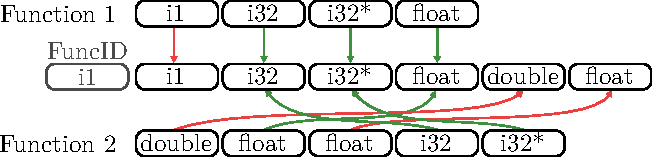
\includegraphics[width=0.9\linewidth]{figs/merged-params.pdf}
  \caption{Example of a merge operation on the list of parameters of two functions.}
  \label{fig:merged-params}
\end{figure}


When multiple available parameters of one function have the same type as a given
parameter from the other function, we choose the one that minimizes the number
%of select instructions by analyzing all pairs of matching instructions in the
%aligned sequence that contain the parameters as operands.
of select instructions.
%We are able to find pairs of parameters that minimize the number of selects by
The pairs of parameters that minimize the number of selects can be found by
analyzing all pairs of matching instructions, in the aligned sequence, that
contain the corresponding parameters as operands.
Experiments show that maximizing the matching of parameters, compared to never
%merging them, improves the average code-size reduction in about 1\%, with
%improvements in individual benchmarks of up to 7\%.
merging them, improves code-size reduction of individual benchmarks by up to 7\%.


%\subsubsection{Control-Flow Graph Reconstruction}

After generating the merged list of parameters, we perform a code generation
to produce the CFG of the merged function in two passes over the aligned
sequence: the first pass creates the basic blocks and instructions,
the second assings the correct operands to the instructions, which also connects
the basic blocks.
A two-passes approach is required in order to handle loops, due to cyclic
dependences.
%Listing~\ref{lst:CodeGen} presents the pseudocode for the code generation.

%\begin{myfloat}[h]
%  \begin{lstlisting}[caption={Pseudocode for the code generation. \todo{simplify.}}, label={lst:CodeGen}]
%CodeGen(Sequence, Function) {
% CFG = Function.NewCFG()
% VMap = Mapping of values to values
% MergedBB = null
% TailBB = Mapping of labels to labels
% //first pass: create CFG and instructions
% for each Entry in Sequence:
%   if Entry is a match:
%      if Entry is of labels:
%         BBLabel = CFG.NewBlock()
%         ValMap[Entry[0]] = BBLabel
%         ValMap[Entry[1]] = BBLabel
%         if Entry has landingPad:
%           create landingpad for BBLabel
%         MergedBB = BBLabel
%      if Entry is of instructions:
%         I0, I1 = Entry[0], Entry[1]
%         if MergedBB is null:
%           MergedBB = G.addBasicBlock()
%           TailBB[I0.getBlock()].addBranch(MergedBB)
%           TailBB[I1.getBlock()].addBranch(MergedBB)
%         add cloned instruction to MergedBB
%         if Entry is terminator instruction:
%           MergedBB = null
%   else:
%      if MergedBB not null:
%        branch to two new basic blocks
%        add new basic blocks to TailBB
%        MergedBB = null
%
%      if Entry is a label:
%        BBLabel = G.NewBlock()
%        ValMap[Entry] = BBLabel
%      if Entry is an instruction:
%        BB = TailBB[Entry.getBlock()]
%        add cloned instruction to the BB
%
% //second pass: update operands
% for each Entry in Sequence:
%   if Entry is a match:
%      if Entry is of instructions:
%         I0, I1 = Entry[0], Entry[1]
%         I = ValMap[I0]
%         
%         for each (Op0, Op1) in I0 and I1:
%           Op0Val = ValMap[Op0]
%           Op1Val = ValMap[Op1]
%           OpVal = Op0Val //assuming equality
%           if ValMap[Op0]!=ValMap[Op1]:
%              OpVal = G.addSelect(Op0Val,Op1Val)
%           update operand of I with OpVal
%   else:
%      if Entry is an instruction:
%        I = ValMap[Entry]
%        update all operands of I using ValMap
%
%}
%  \end{lstlisting}
%\end{myfloat}

First, for each entry in the aligned sequence, we either create a new basic
block for labels or we add a cloned instruction to the appropriate basic
block.
If the label represents a landing block, a landingpad instruction is also added
to the new baisc block.
During this process, we keep a mapping from the instructions and labels in the
original functions to their corresponding values in the new merged function.
This mapping is required in order to appropriately create the use-definition
chains for the merged function, which is done by pointing the operands of the
instructions to the correct values in the function.
However, at this point, the cloned instructions are created with empty operands,
as we are still creating this mapping.

Moreover, while iterating over the aligned sequence, we also need
to create extra basic blocks and branch instructions in order to maintain the
semantics of the original functions.
When transitioning from matching instructions or labels to non-matching ones,
we need to branch to new basic blocks based on the function identifier.
This divergent point is used to continue code generation for the non-matching
segment of the aligned sequence.
When trasitioning back from non-matching segments to a matching segments, then
we need to reconnect both divergent points by branching back to a single new
basic block where merged instructions will be added.

The second pass over the aligned sequence is solely responsible for updating
the operands of cloned instructions and adding select instructions as necessary.
Select instructions are created when a merged instruction has different operand 
values in the original functions, thus the appropriate value needs to be
selected based on the function identifier.
However, if the operands are labels, instead of adding a select instruction,
the operand selection is performed in a control-flow manner, using a new basic
block and a conditional branch based on the function-identifier parameter.
When the two labels represents landing blocks, we hoist the landingpad
instruction to the new common basic block, converting it to a landing block and
converting the two landing blocks to normal basic blocks.
This is required for the correctness of the landing-pad model.
Moreover, similar to previous work on vectorization~\cite{porpodas18}, we also
exploit commutative instructions in order to maximize similarity.
When merging two commutative instructions, we perform operand reordering to
maximize the number of matching operands and reduce the total number of select
instructions added to the merged function.

It is important to note that if we are merging two identical functions, no
select or extra branch instruction will be added.
As a result, we can remove the extra parameter that represents the function
identifier.

\section{A Framework for the Function Merging Optimization}
\label{sec:framework}

In this section, we describe our implementation of the function merging
optimization, which combines the proposed function-merging technique with an
efficient exploration infrastructure.

Although the proposed technique is able to merge any two functions, it is not
always profitable to merge them.
In fact, as it is only profitable to merge functions that are sufficiently
similar, for most pairs of functions, merging them increases code size.
Therefore, the main goal of the exploration infrastructure is to efficiently
find pairs of functions that are profitable to merge.

As described in Section~\ref{sec:background}, LLVM's existing function merging
optimization, due to its hard restriction of only merging identical functions,
is able to  efficiently explore which functions to merge by computing a hash
of the functions.
If two functions have the same hash, they are very likely to be identical.
Moreover, merging identical functions is always profitable.
Because the proposed function-merging technique is able to merge any pair of
functions, we have a much larger exploration space and also a more challenging
decision problem.

%\subsection{Ranking Infrastructure}

For every function, ideally we would like to try to merge with all other
functions and choose the pair that maximizes code reduction.
However, this quadratic exploration over all pairs of functions results in 
compilation-time overheads that are usually unacceptable for real-world
scenarios.
In order to avoid the quadratic exploration of all possible merges, we propose
the framework shown in Figure~\ref{fig:func-merge-opt-arch} for the
function merging optimization.

\begin{figure}[h]
  \centering
  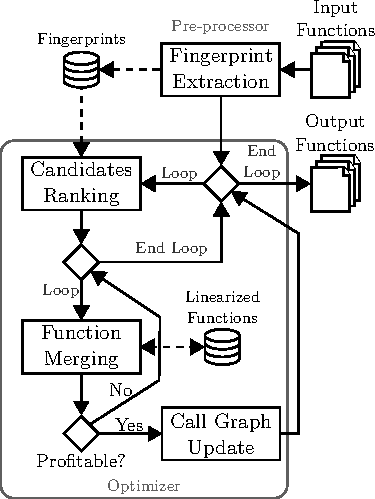
\includegraphics[width=0.7\linewidth]{figs/func-merge-opt-arch.pdf}
  \caption{Overview of the optimization.}
  \label{fig:func-merge-opt-arch}
\end{figure}

The proposed framework is based on a light-weight ranking infrastructure that
uses a \textit{fingerprint} of the functions to evaluate their similarity.
It starts by first precomputing and caching the fingerprint of all functions.
The goal of the fingerprint is to allow us to efficiently discard unpromising
pairs of functions so that we perform the more expensive evaluation only on
the topmost similar pairs.
To this end, the fingerprint consists of: $(1)$ map of instruction opcodes to
the their frequency on the function; $(2)$ the set of types of manipulated by
the function.
While functions can have several thousands of instructions, an IR usually has
just a few tens of opcodes, e.g., the LLVM IR has only about 64 different
opcodes.
This means that the fingerprint needs to store just a small integer array of the
opcode frequencies and a set of types, which allows for an efficient similarty
comparison.

By comparing the opcode frequencies of two functions we are able to estimate
an upper bound of the merge between these functions, assuming that all
instructions with the same opcode would always have a match.
This assumption provides an upper bound on the number of actual matches since
it may be affected by the instruction types and the order they appear in the
sequence.
As a way to refine this estimate, we weight this upper bound by the
type-similarity ratio between the two functions, where we use the Jaccard
similarity coefficient~\cite{jaccard}.
Let $T_1$ and $T_2$ be the set of types of the functions $f_1$ and $f_2$,
respectively.
Therefore, the upper bound reduction, computed as a ratio, can be defined as
\[
   U\!B(f_1,f_2) = \frac{\sum\limits_{op \in Ops} \min\{freq(op,f_1),freq(op,f_2)\}}{\sum\limits_{op \in Ops} freq(op,f_1)+freq(op,f_2)}
\]
and the weighted estimate is given by
\[
     s(f_1,f_2) = U\!B(f_1,f_2) \frac{|T_1 \cap T_2|}{|T_1 \cup T_2|}
\]
This weighted estimate results in a value in the range $[0,0.5]$,
which encodes a description that favors maximizing both the opcode and type
similarities, while minimizing their respective differences.
Identical functions will always result in the maximum value of $0.5$.

For each function $f_1$, we use a priority queue to rank the topmost
similar candidates based on their similarity defined by $s(f_1,f_2)$, for all
other functions $f_2$.
We use an exploration threshold to limit how many top candidates we will
evaluate for any given function.
This cadidate exploration is then performed in a greedy fashion, where the first
candidate that actually results in a profitable merge ends the exploration and
the merge is finally commited.

\begin{figure}[h]
  \centering
  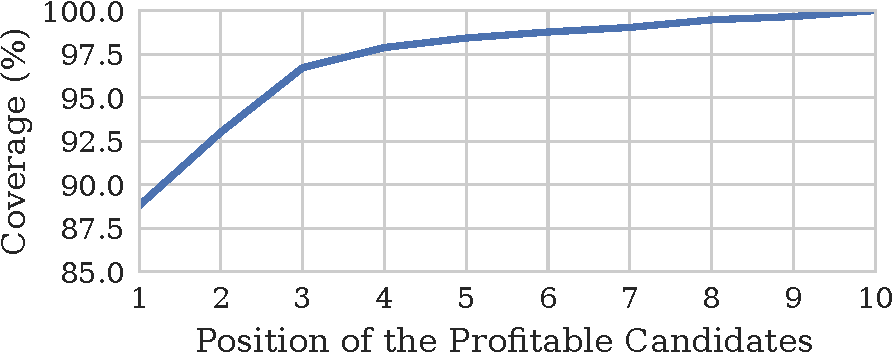
\includegraphics[width=\linewidth]{figs/average-cdf-exploration-threshold.pdf}
  \caption{Average CDF for the exploration threshold and the percentage of merged operations covered.
           A merge operation happens with the topmost candidate in about 89\% of the cases.}
  \label{fig:average-cdf-exploration-threshold}
\end{figure}

Ideally, the profitable candidate will be as close to the top of the rank as
possible.
Figure~\ref{fig:average-cdf-exploration-threshold} shows the cummulative
distribution of the position of the profitable candidates in a top 10 rank.
It shows about 89\% of the merge operations occurred with the topmost candidate,
where the top 5 covers over 98\% of the profitable candidates.
These results suggest that the proposed fingerprint similarity is able to
accuretly capture the real function similarity, while possibly reducing the
exploration cost by a few orders of magnitudes, depending on the actual number
and size of the functions.

When a profitable candidate is found, then we first replace the body of the two
original functions to a single call instruction to the merged function.
Afterwards, if the original functions can be completely removed, we update the
call graph, replacing the calls to the original functions by calls to the 
merged function.
When compiling the whole-program during link-time optimization, we can be more
aggressive when removing the original functions.
However, if the optimization is applied per compilation unit, then extra
conditions must be guaranteed, e.g., the function must not be externally visible
to other compilation units. 
Finally, the new function is added to the optimization working list.
Because of this feedback loop, merge operations can also be performed on
functions that resulted from previous merge operations.
 
\subsection{Profitability Cost Model}

After generating the code of the merged function, we need to estimate the
code-size benefit of replacing the original pair of functions by the new merged
function.
In order to estimate the code-size benefit, we first compute the code-size cost
for each instruction in all three functions.
In addition to measuring the difference in size of the merged function, we also
need to take into account the extra costs:
$(1)$ for the cases where we need to keep the original functions with a call to
the merged function;
and $(2)$ for the cases where we update the call graph, there might be an extra
cost with a call to the merged function due to the increased number of arguments.

Let $c(f)$ be the code-size cost of a given function $f$, and
$\delta(f_i, f_j)$ represent the extra costs involved when replacing or
updating function $f_i$ with the function $f_j$.
Therefore, given a pair of functions $\{f_1,f_2\}$ and the merged function
$f_{1,2}$, we want to maximize the profit defined as:
\[
  \Delta(\{f_1,f_2\},f_{1,2}) = (c(f_1)+c(f_2)) - (c(f_{1,2}) + \varepsilon)
\]
where $\varepsilon = \delta(f_1, f_{1,2}) + \delta(f_2, f_{1,2})$.
We consider that the merge operation is profitable if $\Delta(\{f_1,f_2\},f_{1,2})>0$.

However, because we are operating on the IR level, one IR instruction does not
necessarily translate to one machine instruction.
Because of that, the profitability is measured with the help of the compiler's
target-spcific cost model.
The actual cost of each instruction comes from querying this compiler's built-in
cost model, which provides a target-dependent cost estimation that approximates
the cost of an IR instruction when lowered to machine instructions.
Our implementation makes use of the code-size costs provided by LLVM's
target-transformation interface (TTI), which is widely used in the decision
%making by most of the LLVM's optimizations.
making of most optimizations.
